% mnras_template.tex 
%
% LaTeX template for creating an MNRAS paper
%
% v3.0 released 14 May 2015
% (version numbers match those of mnras.cls)
%
% Copyright (C) Royal Astronomical Society 2015
% Authors:
% Keith T. Smith (Royal Astronomical Society)

% Change log
%
% v3.0 May 2015
%    Renamed to match the new package name
%    Version number matches mnras.cls
%    A few minor tweaks to wording
% v1.0 September 2013
%    Beta testing only - never publicly released
%    First version: a simple (ish) template for creating an MNRAS paper

%%%%%%%%%%%%%%%%%%%%%%%%%%%%%%%%%%%%%%%%%%%%%%%%%%
% Basic setup. Most papers should leave these options alone.
\documentclass[fleqn,usenatbib]{mnras}

% MNRAS is set in Times font. If you don't have this installed (most LaTeX
% installations will be fine) or prefer the old Computer Modern fonts, comment
% out the following line
\usepackage{newtxtext,newtxmath}
% Depending on your LaTeX fonts installation, you might get better results with one of these:
%\usepackage{mathptmx}
%\usepackage{txfonts}

% Use vector fonts, so it zooms properly in on-screen viewing software
% Don't change these lines unless you know what you are doing
\usepackage[T1]{fontenc}
% Allow "Thomas van Noord" and "Simon de Laguarde" and alike to be sorted by "N" and "L" etc. in the bibliography.
% Write the name in the bibliography as "\VAN{Noord}{Van}{van} Noord, Thomas"
\DeclareRobustCommand{\VAN}[3]{#2}
\let\VANthebibliography\thebibliography
\def\thebibliography{\DeclareRobustCommand{\VAN}[3]{##3}\VANthebibliography}


%%%%% AUTHORS - PLACE YOUR OWN PACKAGES HERE %%%%%
\usepackage{tabularx}
% Only include extra packages if you really need them. Common packages are:
\usepackage{graphicx}	% Including figure files
\usepackage{amsmath}	% Advanced maths commands
%\usepackage{amssymb}	% Extra maths symbols
\usepackage{subfig}
% \usepackage{cleveref}
\usepackage[capitalise]{cleveref}
\usepackage{hyperref}
%%%%%%%%%%%%%%%%%%%%%%%%%%%%%%%%%%%%%%%%%%%%%%%%%%

%%%%% AUTHORS - PLACE YOUR OWN COMMANDS HERE %%%%%

% Please keep new commands to a minimum, and use \newcommand not \def to avoid
% overwriting existing commands. Example:
%\newcommand{\pcm}{\,cm$^{-2}$}	% per cm-squared

%%%%%%%%%%%%%%%%%%%%%%%%%%%%%%%%%%%%%%%%%%%%%%%%%%


%%%%%%%%%%%%%%%%%%% TITLE PAGE %%%%%%%%%%%%%%%%%%%

% Title of the paper, and the short title which is used in the headers.
% Keep the title short and informative.
\title[Bayesian Approach to RFI Mitigation]{A Bayesian approach to RFI mitigation}

% The list of authors, and the short list which is used in the headers.
% If you need two or more lines of authors, add an extra line using \newauthor
\author[S.A.K Leeney et al.]{
S.A.K. Leeney,$^{1}$\thanks{E-mail: sakl2@cam.ac.uk (KTS)}
W.J. Handley,$^{1, 2}$
E. de Lera Acedo$^{1, 2}$
\\
% List of institutions
$^{1}$Astrophysics Group, Cavendish Laboratory, J. J. Thomson Avenue, Cambridge, CB3 0HE, UK\\
$^{2}$Kavli Institute for Cosmology, Madingley Road, Cambridge, CB3 0HA, UK\\
}

% These dates will be filled out by the publisher
\date{Accepted XXX. Received YYY; in original form ZZZ}

% Enter the current year, for the copyright statements etc.
\pubyear{2022}

% Don't change these lines
\begin{document}
\label{firstpage}
\pagerange{\pageref{firstpage}--\pageref{lastpage}}
\maketitle

% Abstract of the paper
\begin{abstract}
Radio Frequency Interference (RFI) is an endemic problem in radio astronomy. Information in contaminated frequency channels is lost and it can lead to significant systematic error if not properly modelled. In this paper we propose a RFI mitigation methodology that takes a Bayesian approach, where contaminated data is both flagged and managed as part of a single step fitting process. To the authors knowledge, our approach is first-of-its-kind. We provide a proof-of-concept of our methods which are also tested and shown to be effective on both a simple toy model and when incorporated into the Bayesian data analysis pipeline for REACH (a modern cosmological radio experiment). 
\end{abstract}

% Select between one and six entries from the list of approved keywords.
% Don't make up new ones.
\begin{keywords}
methods: data analysis — methods: statistical
\end{keywords}

%%%%%%%%%%%%%%%%%%%%%%%%%%%%%%%%%%%%%%%%%%%%%%%%%%

%%%%%%%%%%%%%%%%% BODY OF PAPER %%%%%%%%%%%%%%%%%%

\section{Introduction}
The field of radio astronomy is growing rapidly. Since the year 2000, the number of known radio sources has grown from a few hundred thousand to over two million. This is expected to increase further to 70 million with the development of the ASKAP-EMU~\cite{johnston2008science} telescope, and beyond with the development of the SKA~\cite{bourke2015advancing}. Furthermore, global 21cm experiments such as EDGES ~\cite{bowman2018absorption},  REACH~\cite{de2022reach} and SARAS~\cite{singh2017first} aim to probe into yet unseen redshift ranges to gain knowledge on the Cosmic Dawn, Dark Ages and Re-ionisation Era.

A major constraint on the design of all such telescopes is radio frequency interference (RFI), which is typically orders of magnitude brighter in amplitude than the sky signal and cannot be modelled as Gaussian noise. RFI is typically anthropogenic, narrow band and comes in various species that can be either constant in time or transient~\cite{ellingson2006rfi}. Sources of RFI include FM Radio and Digital TV signals. 

Building antennae in remote locations on earth can alleviate but never completely avoid such nuisance signals. Furthermore, RFI always increases the amplitude of the detected signal and is often transient in nature. Therefore, simply averaging the sky over long time spans (for example in global experiments) is not sufficient to prevent contaminated data leading to systematic errors.

Currently, RFI is flagged and then excised prior to and separately from the data analysis stage of of the radio experiment. In older telescopes this may have been done manually by the astronomer. However with modern telescopes gathering terabytes of data per second, an automated approach is required. Various approaches have been taken in the past including wavelet based methods~\cite{oslick1998general}, \textsc{cumsum}~\cite{baan2004radio}, and the \textsc{aoflagger}~\cite{offringa2010aoflagger} package used for LOFAR, which implements Singular Value Decomposition~\cite{offringa2010post}. Another approach, used by the HERA project, is to flag the data using a watershed segmentation algorithm~\cite{kerrigan2019optimizing}. More recently, Deep Learning models using convolutional neural networks trained on manually flagged and/or and simulated data~\cite{akeret2017radio};~\cite{vafaei2020deep};~~\cite{sun2022robust} have been shown to be able to effectively flag varying species of RFI. \cite{kennedy2022statistical} takes a partially Bayesian approach where contaminated frequency channels are flagged and then excised using other methods, after which they are mitigated for using  Gaussian constrained realisations and Gibbs sampling.

In this paper we propose a first-of-its-kind RFI mitigation algorithm that takes a Bayesian Approach, where RFI is both flagged and managed at the likelihood level. The paper is structured as follows: we introduce the basic theory behind Bayesian Inference in~\cref{sec:bayesianinftheory}; then we introduce our Bayesian RFI Correction method in~\cref{sec:rficorrtheory}; followed by an analysis of the model when tested on a simple toy scenario in~\cref{sec:toyex}; our methodology is then tested in a real use case in the REACH pipeline in~\cref{sec:reachex}; finally we discuss our conclusions in \cref{sec:conclusions}. The techniques described in this paper can be incorporated into a Bayesian data analysis pipeline with just a few lines of code.


\section{Theory}
\subsection{Bayesian Inference}\label{sec:bayesianinftheory}
Bayesian methods can be used to perform parameter estimates and model comparison. A model $\mathcal{M}$ uses data $\mathcal{D}$ to infer its free parameters $\theta$. Using Bayes Theorem,
\begin{align}
    P(\mathcal{D}|\theta) \times P(\theta) &= P(\theta|\mathcal{D}) \times P(\mathcal{D}), \\
    \mathcal{L} \times \pi &= \mathcal{P} \times \mathcal{Z},
\end{align}
the prior $\pi$ is updated onto the posterior $\mathcal{P}$ in light of the likelihood $\mathcal{L}$ and furthermore the Bayesian Evidence $\mathcal{Z}$ can be inferred by computing the integral
\begin{equation}
    \mathcal{Z} = \int \mathcal{L}(\theta) \times \pi(\theta) \; d\theta.
\end{equation}
In practice, $\mathcal{P}$ and $\mathcal{Z}$ can be determined simultaneously using a Bayesian numerical solver. We use the Nested Sampling algorithm \textsc{polychord}~\cite{handley2015polychord}; where a series of points generated within $\pi$ are updated such that they sequentially contract around the peak(s) of the likelihood, forming the posterior which can be used to generate parameter estimates. The artefacts of this process can then be used to compute $\mathcal{Z}$, which is used for model comparison. For a more detailed description of Bayesian Inference and Nested Sampling see \cite{sivia2006data}.

\subsection{RFI correction likelihood}\label{sec:rficorrtheory}
A data point contaminated by RFI can be considered corrupted. Any information relevant to the model is lost and furthermore it cannot be modelled as Gaussian noise. Assuming $\mathcal{D}$ is uncorrelated, the likelihood
\begin{equation}
\begin{aligned}
   \mathcal{L} &= P(\mathcal{D}|\theta) = \prod_{i} \mathcal{L}_{i}(\theta),\label{l1} = \prod_{i} P(\mathcal{D}_i|\theta)
\end{aligned}
\end{equation}
where $i$ represents the $i$'th data point, is insufficient to model such contaminated data.
It is therefore necessary to model the likelihood that each data point is corrupted. 

Thus, we introduce a piecewise likelihood including the possibility of corruption of data
\begin{equation}
    P(\mathcal{D}_i|\theta) = \begin{cases}
        \mathcal{L}_i(\theta) &: \text{uncorrupted}\\
        \Delta^{-1}[ 0<\mathcal{D}_i<\Delta] &: \text{corrupted}.\\
    \end{cases}
\end{equation}
Corruption is modelled as the data becoming completely unreliable and therefore being distributed uniformly within some range $\Delta$ (which, as a scale of corruption, has the same dimensions as the data).
An efficient way to write this likelihood is
\begin{equation}
    P(\mathcal{D}|\theta, \varepsilon) = \prod_{i} \mathcal{L}_{i}^{\varepsilon_{i}} \Delta^{\varepsilon_i-1}
    \label{eq:li2}
\end{equation}
where the Boolean mask vector $\varepsilon$ has a $i$th component which takes the value $1$ if the datum $i$ is uncorrupted and value $0$ if corrupted.

We do not know before the data arrive whether or not they are corrupted by RFI. We may infer this in a Bayesian fashion, by ascribing a Bernoulli prior probability $p_i$ of corruption (which has dimensions of probability) i.e:
\begin{equation}
P(\varepsilon_i) = p_i^{(1-\varepsilon_i)}(1-p_i)^{\varepsilon_i}.\label{eq:pei}
\end{equation}
Both $\Delta$ and $p_i$ are required for a dimensionally consistent analysis. It should be noted that above we assume the a-priori probability that each bin contains RFI is uncorrelated, i.e $P(\varepsilon)=\prod _i P(\varepsilon_i)$, which in practice will almost certainly not be true. We will discuss later the extent to which this assumption can be considered valid.

Multiplying \cref{eq:pei,eq:li2} yields
\begin{equation}
    P(\mathcal{D},\varepsilon|\theta) = \prod_{i} \left[\mathcal{L}_{i}(1-p_i)\right]^{\varepsilon_{i}} \left[p_i/\Delta\right]^{(1-\varepsilon_i)}
    \label{eqn:likelihood_eps}
\end{equation}
and to recover a likelihood independent of $\varepsilon$ we formally can marginalise out:
\begin{align}
    P(\mathcal{D}|\theta) &=\sum_{\varepsilon \in \{ 0, 1 \} ^N}P(\mathcal{D},\varepsilon|\theta) \\
    &= \sum_{\varepsilon \in \{ 0, 1 \} ^N} \prod_{i} \left[\mathcal{L}_{i}(1-p_i)\right]^{\varepsilon_{i}} \left[p_i/\Delta_i\right]^{(1-\varepsilon_i)}.
    \label{eq:pdtheta2}
\end{align}
This would require the computation of the all $2^N$ terms in \cref{eq:pdtheta2}. For realistic values of $N$, this computation becomes impractical. However, if it is assumed that the most likely model (i.e the maximum term in \cref{eq:pdtheta2}) dominates over the next to leading order terms, we can make the approximation
\begin{equation}
    P(\mathcal{D},\varepsilon|\theta) \approx \delta_{\varepsilon \varepsilon^\mathrm{max}} \times P(\mathcal{D},\varepsilon^{\mathrm{max}}|\theta)\label{eqn:postierioreps}
\end{equation}
where $\delta_{ij}$ is the usual Kroneker delta function, and
 $\varepsilon^\mathrm{max}$ is the mask vector which maximises the likelihood $P(D,\varepsilon|\theta)$, namely:
\begin{equation}
    \varepsilon^{\mathrm{max}}_{i}=
    \begin{cases}
        1, & \mathcal{L}_i(1-p_i) > p_i/\Delta_i \\
        0, & \text{otherwise}.
    \end{cases}
    \label{eqn:emax}
\end{equation}
Under this approximation we find that the sum in \cref{eq:pdtheta2} becomes
\begin{equation}
    P(\mathcal{D}|\theta) \approx P(\mathcal{D},\varepsilon^{\mathrm{max}}|\theta).\label{eq:approx}
\end{equation}

In practice the approximation in \cref{eq:approx} is only valid if the next to leading order term is much smaller, such that
 \begin{equation}
 P(\mathcal{D}|\theta, \varepsilon_{\mathrm{max}}) \gg \mathrm{max}_j P(\mathcal{D}|\theta,\varepsilon^{(j)})\label{eq:nlo},
\end{equation}
where $\varepsilon^{(j)}$ is $\varepsilon^\mathrm{max}$ with its $j$th bit flipped:
\begin{equation}
    \varepsilon^{(j)}_k = 
    \begin{cases}
    1-\varepsilon^{\mathrm{max}}_k & k=j \\
    \varepsilon^{\mathrm{max}}_k & k\ne j \\
\end{cases}
\end{equation}
and we may use \cref{eq:nlo} as a consistency check.

To summarise, we can correct for RFI under these approximations by replacing the original likelihood $\mathcal{L} = \prod_i\mathcal{L}_i$ in \cref{l1} with 
\begin{equation}
    P(\mathcal{D}|\theta) = \prod_i\left[\mathcal{L}_{i}(1-p_i)\right]^{\varepsilon^{\mathrm{max}}_{i}} \left[p_i/\Delta\right]^{(1-\varepsilon^\mathrm{max}_i)}
    \label{eqn:likelihood}
\end{equation}
where $\varepsilon^{\mathrm{max}}$ is defined by \cref{eqn:emax}.
\subsection{Computing the posterior}
The posterior and evidence are computed from \cref{eqn:likelihood} via Nested Sampling (although any numerical Bayesian sampling method could be used). Taking logs for convenience gives
\begin{equation}
    \begin{aligned}
        \log{P(\mathcal{D}|\theta)} = \sum_{i} &[\log{\mathcal{L}_i}+\log({1-p_i})]\varepsilon^{\mathrm{max}}\\ 
        &+ [\log{p}_i - \log{\Delta}](1 - \varepsilon^\mathrm{max}_i), \label{eq:loglikelihood}
    \end{aligned}
\end{equation}
yielding a masked chi squared like term which can be used to distinguish whether there is a statistically significant difference between the classes of data, i.e corrupted or non corrupted. Furthermore, the second term in \cref{eq:loglikelihood} introduces an Occam penalty. Each time a data point is predicted to be RFI its likelihood is replaced with the penalty rather than being completely removed. Without this term, the likelihood where all data points are flagged would be larger and thus `more likely' than all other possibilities. Therefore, flagging all datum would always be preferable.

We compute this by imposing the condition in \cref{eqn:emax} on \cref{eq:loglikelihood} as follows, \begin{equation}
    \log{P(\mathcal{D}|\theta)} =  
    \begin{cases}
        \log \mathcal{L}_i + \log (1-p_i), &
    \begin{aligned}
        &[\log{\mathcal{L}_i} + \log({1-p_i}) \\
        &> \log p_i - \log \Delta]
    \end{aligned}\\ 
        \log p_i - \log \Delta, & \text{otherwise}.
    \end{cases}
    \label{eqn:loglcompute}
\end{equation}
The effect that this correction has on a log-likelihood with a corrupted datapoint is shown in \cref{fig:theorysketch}.

The corrected likelihood is then updated iteratively via the selected Bayesian sampling method, compressing the prior onto the posterior while simultaneously correcting for RFI. One may also notice that the right hand side of \cref{eq:loglikelihood} is a Logit function. Logit functions are used routinely as an activation function in binary classification tasks, which hints at the potential of a future extension of this work using machine learning.

\begin{figure}
	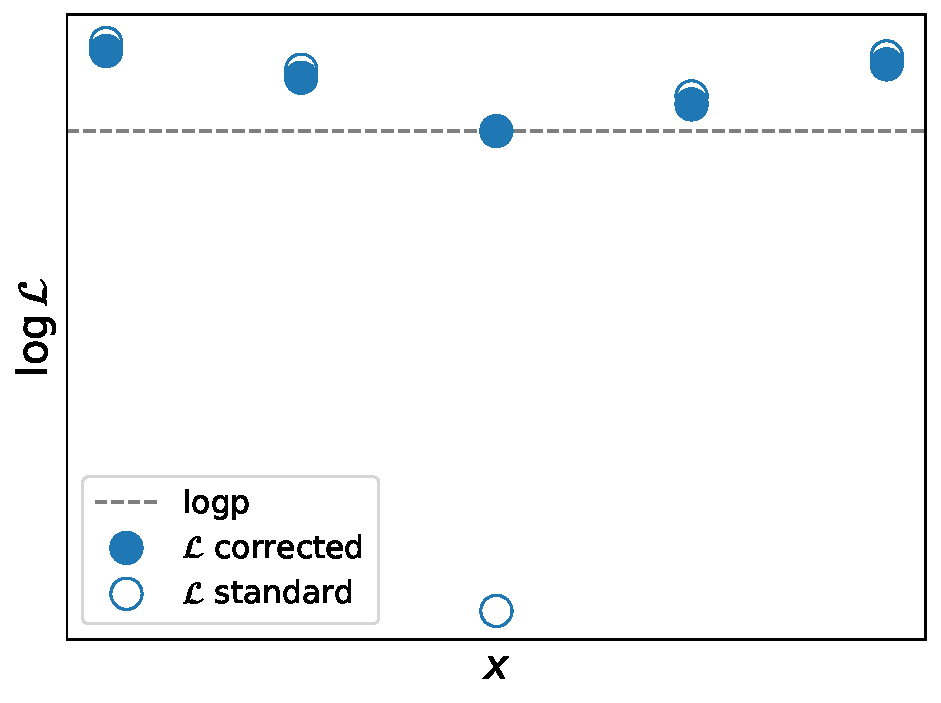
\includegraphics[width=\columnwidth]{f_theory_sketch.pdf}
    \caption{Visualising the effect of a correction on the likelihood for a simple 5 point data set where the 3rd point is corrupted.}
    \label{fig:theorysketch}
\end{figure}
\section{Toy Example}\label{sec:toyex}
We will initially test this approach on a simple toy model, consisting of a straight line with Gaussian noise and RFI injected. Then, we move onto a more realistic and complex case in \cref{sec:reachex}.
\subsection{Dataset}\label{sec:toyexdataset}
Two datasets of 25 data points are generated for comparison. The first is a line with Gaussian noise $\sigma=5$, gradient $m=1$ and intercept $c=1$. It does not contain RFI thus can be used as a ground truth. The second dataset is the same, with the random noise identically seeded so the data is reproducible, but with two RFI spikes injected. This is shown in the top pane of \cref{fig:posterior_frac_toy}.

\subsection{Initial Testing}\label{sec:initialsetup}
We fit the data described in \cref{sec:toyexdataset} in a Bayesian sense and attempt to recover the two free parameters $m$ and $c$ using the correcting likelihood in \cref{eqn:loglcompute} with
\begin{equation}
\mathcal{L}_i = -\frac{\log(2\pi \sigma^{2})}{2} - \frac{[y_{i} - y_{\mathcal{S}}(x_i;m, c)]^2}{2\sigma^2},
\end{equation}
where $\theta = m, c, \sigma$, $y_i$ is the simulated data and $y_\mathcal{S}(x_i; m, c)$ is the output when the estimated parameters from the current sampling iteration are used to compute the model $y_i=mx_i + c$. We set $\Delta = \mathcal{D}_\textsc{max}$, to encapsulate the full range of possible data values. $\Delta$ could likely be fit as a free parameter, as will be investigated further in future works.

Sampling the posterior $P(\theta|\mathcal{D})$ via a Bayesian sampling procedure, the prior distribution is compressed and the belief that each point fits (or is corrupted and does not fit) the model is updated. Thus by evaluating the subsequent posterior on $\varepsilon$, as shown in \cref{fig:posterior_frac_toy}, we can assess how many times across the entire sampling run each data point was believed to fit (non corrupted) or not fit (corrupted) the model. As seen in \cref{fig:posterior_frac_toy}, it is evident that the points containing RFI make up a near zero fraction of the posterior, because as the prior was iteratively updated onto the posterior they were frequently believed to be corrupted. Conversely, points that do not contain RFI often fit the model and as such contribute significantly to the final posterior distribution. There are also some points that lie somewhere in between, which the model is less confident are uncontaminated. When comparing the data in the top pane to the bottom pane in the probability domain, it appears as though the points the model has less confidence in are the ones that deviate the most from the true signal due to Gaussian noise. 
\begin{figure}
	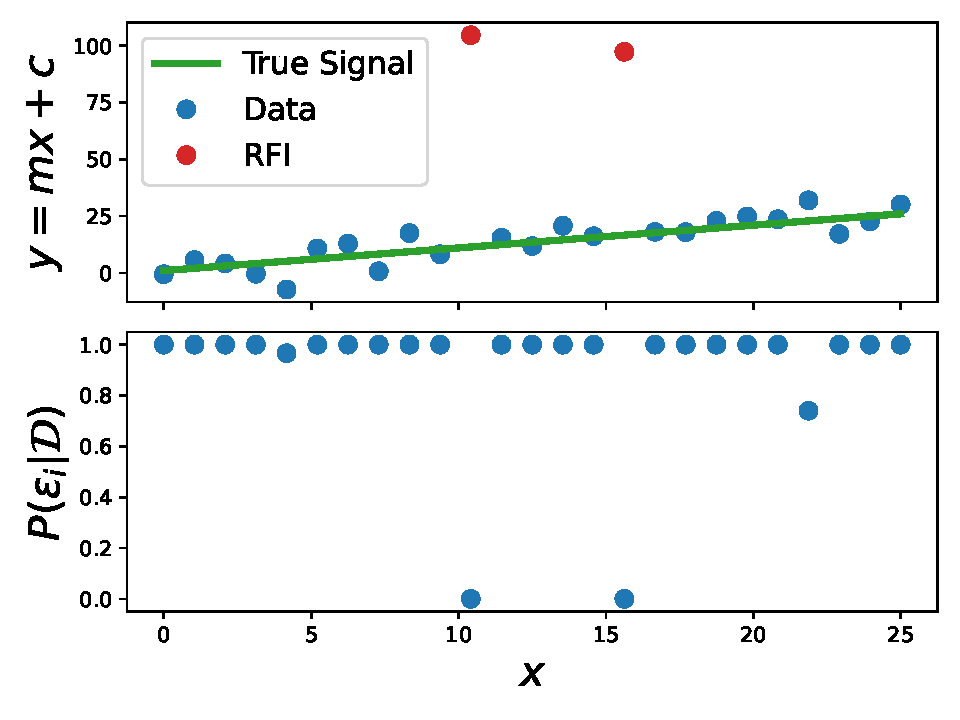
\includegraphics[width=\columnwidth]{f_test.pdf}
    \caption{The top pane shows the dataset described in~\cref{sec:toyexdataset}, with the true signal marked in green and points corrupted by RFI marked in red. The bottom pane shows the mean posterior on $\varepsilon$, $P(\varepsilon_i|\mathcal{D})$, produced during the sampling run.}
    \label{fig:posterior_frac_toy}
\end{figure}
It should be emphasised that although $\varepsilon_i$ is constrained to binary values, the subsequent mask on $\varepsilon$ is not. Unlike traditional RFI flagging algorithms, points are not simply flagged as  `RFI' and `Not RFI'. The mask takes the weighted mean across the posterior. Thus, points more likely to contain RFI will have less `impact' on the final posterior distribution than points believed to be uncontaminated. In practice, as seen in \cref{fig:posterior_frac_toy}, points predicted to contain RFI will have a near zero contribution on the subsequent posterior. However, it is possible that points which the model is less confident in, such as at $x=4$ and $x=22$ will have a lesser but non-zero contribution to the final distribution. The mask could be thought of as being slightly opaque to these data points, accounting for the models uncertainty. The ability to incorporate the models confidence in its correction directly into the subsequent parameter estimates and model comparison makes this mitigation approach unique in comparison with its counterparts. 
\subsection{Model Evaluation}
To further examine the effectiveness of the our methodology it is necessary to develop a simple toy model, similar to the above but also simulating various other scenarios. Both datasets described in \cref{sec:toyexdataset} will be evaluated when fit using the likelihood capable of correcting for RFI. They will also be fit using a traditional likelihood, which cannot account for RFI. This will generate a total of four posterior distributions for comparison. 

We initially fit a baseline case to be used as a ground truth, using the clean dataset and a traditional likelihood that does not facilitate the modeling of RFI. The new likelihood which is capable of correcting for RFI is then used to fit the clean dataset, to confirm that it performs correctly even in the absence of RFI. The dataset containing RFI is then fit using the new likelihood and the traditional likelihood, to examine how much better the model performs when the correction is applied. All but the contaminated, uncorrected case would be expected to perform similarly if RFI has been effectively mitigated. It should be noted however that from a Bayesian standpoint, the simplest model will always be preferable. Thus, for the clean dataset it would be expected that the standard likelihood would be preferred slightly over the correcting likelihood. 

Fig.~\ref{fig:anesthetic} shows the parameter distributions inferred from the data in \cref{sec:toyexdataset} in the four cases described above and their associated $1\sigma$ and $2\sigma$ confidences. The bottom left pane shows that both $m$ and $c$ are inferred to within $1\sigma$ of their true values. The `No RFI No Correction' case is similar to the `RFI Corrected' case, indicating that the model has effectively corrected the corrupted regions of data. This is particularly evident when comparing these two cases to the uncorrected, contaminated case.

According to Bayes theorem, the simplest model will always be favoured. This is clear when comparing the Bayes Factor computed from the log evidences in~\cref{tab:tab1}. For the uncontaminated data, the model that does not correct for RFI is slightly preferred. Conversely the correcting model is strongly preferred on the contaminated data indicating that the correction is working effectively. 
\begin{table}
\begin{center}
\begin{tabularx}{0.4\textwidth} { 
  | >{\raggedright\arraybackslash}X 
  | >{\centering\arraybackslash}X 
  | >{\raggedleft\arraybackslash}X | }
 \hline
   & No RFI & RFI \\
 \hline
 No Correction ($\log \mathcal{Z}$) & -83.9 $\pm$ 0.2  & -120 $\pm$ 0.4 \\
 \hline
 Correction ($\log \mathcal{Z})$ & -85.3 $\pm$ 0.2 & -95 $\pm$ 0.2 \\
 \hline
 $\log$ Bayes Factor & -1.4 $\pm$ 0.3 & 25.0 $\pm$ 0.4 \\
 \hline
\end{tabularx} \label{tab:tabletoymodel}
\caption{Evidences when running the four cases described in~\cref{sec:toyex} and the subsequent Bayes factor.}
\end{center}
\label{tab:tab1}
\end{table}
\begin{figure*}
	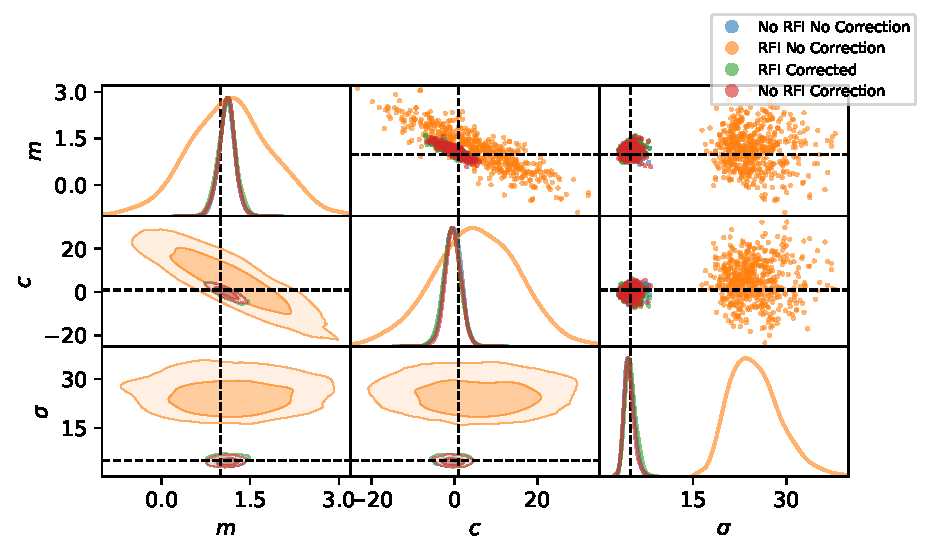
\includegraphics[width=\textwidth]{f_4pane_samples2.pdf}
    \caption{Showing the parameter distributions inferred from the dataset described in Section~\ref{sec:toyexdataset}. The top left to bottom right panes show probability distribution functions for $m$, $c$ and $\sigma$, respectively. Plots generated using  posterior plotting tool \textsc{anesthetic}~\protect\cite{anesthetic}.}
    \label{fig:anesthetic}
\end{figure*}
\begin{figure*}
	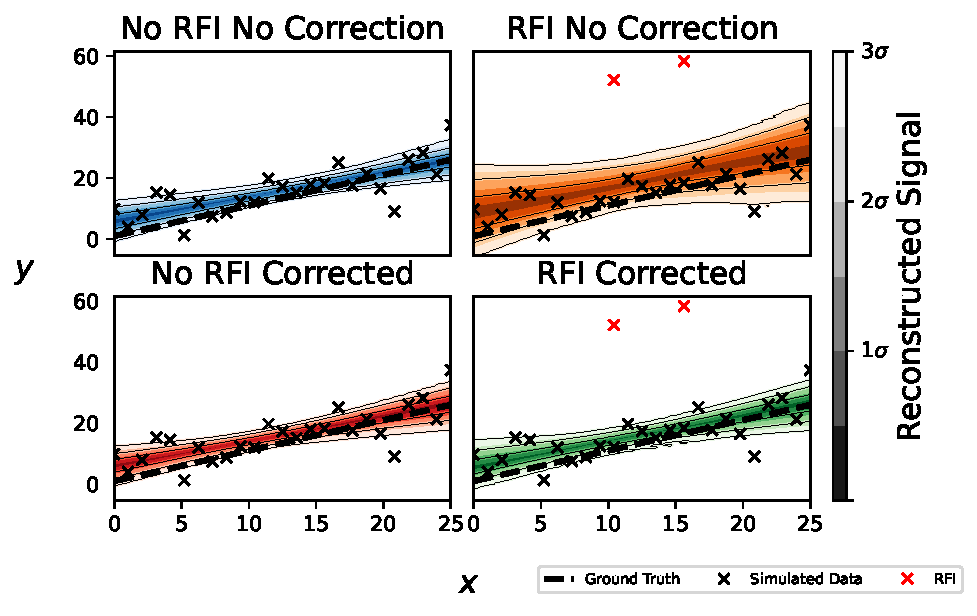
\includegraphics[width=\textwidth]{f_4pane_toy_sidebar.pdf}  
    \caption{Showing the inferred parameter estimates in a contour plot, where darker tones indicate higher $\sigma$ confidence in the parameter estimates. Generated from the dataset described in Section~\ref{sec:toyexdataset}. The plots are generated using the functional posterior plotter \textsc{fgivenx}~\protect\cite{fgivenx}.}
    \label{fig:fgx}
\end{figure*}


It is also useful to view the posterior plots of $P(y|x, \mathcal{D})$ plotted from the inferred parameter estimates and the associated confidences. As seen in \cref{fig:fgx}, when RFI is not corrected, the true value is well outside the $1\sigma$ and sometimes $2\sigma$ confidence bounds. Conversely the other three cases fit almost entirely within the $1\sigma$ bounds, indicating that the RFI has been mitigated.

\subsection{Evaluating the $\log p$ dependence}\label{sec:logpdependence}
Proper selection of the probability thresholding term $\log p$ is essential to the efficacy of the mitigation process. Set too high, the model will require such a high confidence of a data point fitting the model that deviations due to Gaussian noise will be predicted as RFI. Set too low, nothing will be corrected. From a Bayesian standpoint $\log p$ would be set to represent our prior degree of belief in there being RFI in each datum.

We firstly assess the question in a qualitative manor, viewing the posterior on $\varepsilon_{\mathrm{max}}$ for a selection of $p $ values. This is computed by evaluating $P(\mathcal{D}|\theta, \varepsilon_{\mathrm{max}})$, avoiding the sum to preserve each data point in $x$ for each posterior sample. We then weighted average across the samples, giving the probability that each data point fits the model. More specifically, the probability that each data point is uncontaminated by RFI. 

When $\log p$ is set appropriately as seen in the left pane of \cref{fig:tri_plot}, the model has a high confidence in its predictions. Across the sampling run the probability threshold frequently laid between the likelihood for contaminated and uncontaminated datapoints, whilst not being so high (and therefore sensitive) as to flag any deviations caused by higher order Gaussian noise. At $\log p = -3.0$ the RFI still appears to have been accurately modelled, however the confidence in some of the predictions are lower. As $\log p$ decreases further, the model breaks down. Points are predicted incorrectly in many of the sampling iterations and as such the model is less able to confidently predict their class. Viewing \cref{fig:tri_plot} from left to right, we observe the effects of this thresholding term moving to the peak of the likelihood, sweeping up points the model is less confident in due to Gaussian noise.
\begin{figure}
	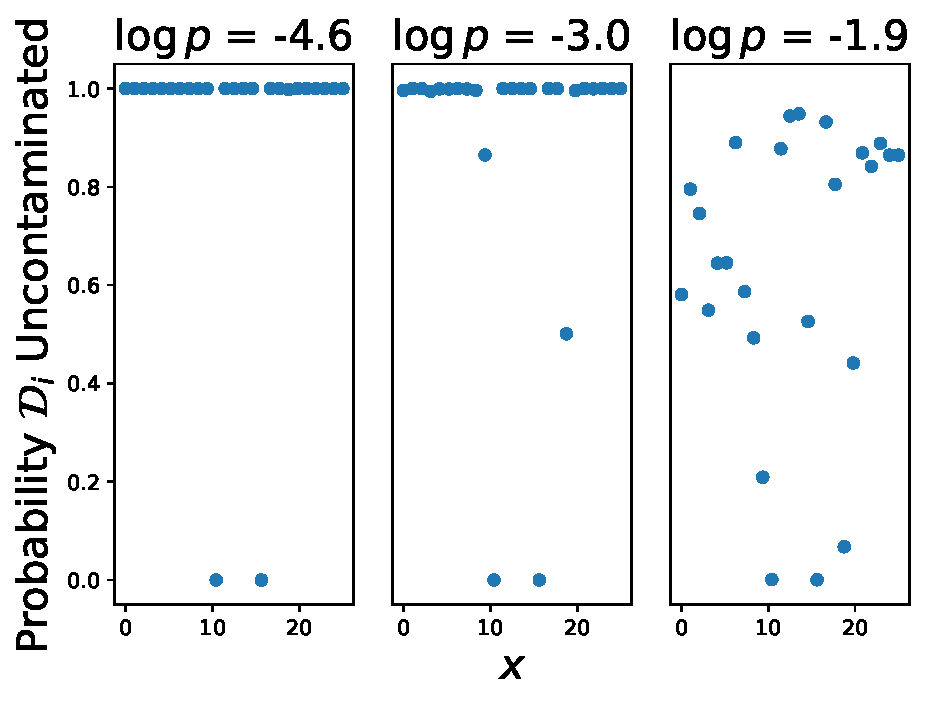
\includegraphics[width=\columnwidth]{f_tri_plot_3_horiz.pdf}
    \caption{Showing the mean mask on $\varepsilon$, ie $P(\varepsilon_i|\mathcal{D})$, where $\log p$ is varied to the point at which the model breaks down.}
    \label{fig:tri_plot}
\end{figure}
We assess the $\log p$ dependence while varying $\log p$ as a function of the RMSE on the fit generated from the parameter estimates, the $\log$ Bayesian Evidence and the mean number of points flagged across all samples. 

\begin{figure}
	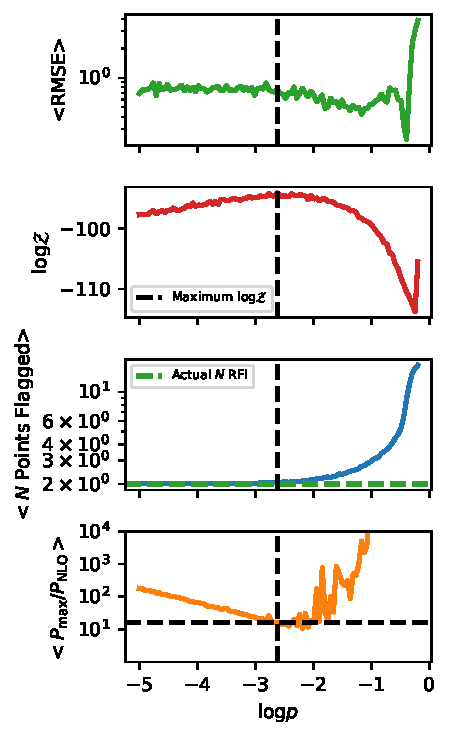
\includegraphics[width=\columnwidth]{f_approx_current_sig5_2.pdf}
    \caption{Assessing how various methods of model evaluation vary as function of $\log p$. From top to bottom: the RMSE, the $\log$ of the Bayesian Evidence, then the weighted average number of points flagged and finally the radio between $P_{\textsc{max}}$ and $P_{\textsc{NLO}}$. All dependant variables (excluding $\log \mathcal{Z}$) are averaged over the weighted posterior samples. The noise observable in these plots is sampling noise; the noise in the simulated data is seeded.}
    \label{fig:4pane}
\end{figure}

For high $\log p$, the RMSE is high and we observe in \cref{fig:4pane} that the model generates less accurate parameter estimates. Here the threshold is so high that the model is more confident that any of the points are RFI than non RFI. This matches the corresponding low evidence. The RMSE drops as $\log p$ decreases to near its minimum. The model incorrectly flags $\approx 5$ data points while the RMSE is low, showing that the model is able to generate accurate parameter estimates whilst over flagging, indicating it is insensitive to false positives. As $\log p$ decreases further, the model is better able to distinguish between higher order Gaussian noise and as such the average number of points predicted to be RFI approaches the true value. As this happens the evidence also reaches its maximum, which indicates that the Bayesian Evidence is appropriately showing how well each of the many models created by different $\log p$ values fit the data.

\subsection{To what extent is $P(\mathcal{D}|\theta) \approx P(\mathcal{D}|\theta, \varepsilon_{\mathrm{max}})$ valid?}
A key assumption is made in \cref{eq:approx} is that the leading order term, \cref{eq:loglikelihood}, is considerably larger than all the other possible terms for $\varepsilon \in (0, 1)^N$. If this approximation is not valid, the mathematical framework behind this approach breaks down.

Therefore it is necessary to test the validity of this approximation by computing \cref{eqn:loglcompute} and comparing the result ($P_{\textsc{max}}$) with the next leading order term ($P_{\textsc{NLO}}$) as calculated by \cref{eq:nlo}. For $-5 < \log p < -0.1$. These results are displayed in the bottom pane of \cref{fig:4pane}. $P_{\textsc{max}}$ is 18 times larger than $P_{\textsc{NLO}}$ at peak $\log \mathcal{Z}$ and increases linearly for $\log p$ below this. Depending on the $\log p$ selection strategy, $P_{\textsc{max}}$ is at least 11 times more likely than the next leading order term. Assuming an appropriate $\log p$ selection strategy, the ratio would be higher, indicating that $P(\mathcal{D}|\theta) \approx P(\mathcal{D}|\theta \varepsilon_{\mathrm{max}})$ is valid.

\subsection{Selection Strategy for $\log p$}
Various selection strategies could be taken to select the optimal $\log p$ value. For each $\log p$, the model changes. As such, selecting the $\log p$ that maximises the evidence seems to be the most obvious selection strategy. In the case of the toy model, the peak $\log \mathcal{Z}$ occurs where $\log p = -2.7$ as shown in \cref{fig:4pane}. Here, $P_{\textsc{max}}$ is 18 times larger than $P_{\textsc{NLO}}$. Another possible strategy could be to select $\log p$ where the number of points flagged is at its minimum. 

It is also possible to ascribe a prior to $\log p$, fitting it as a free parameter thus fully automating the approach. This will be examined further in future works.
\vfill
\section{REACH Example}\label{sec:reachex}
\begin{figure*}
	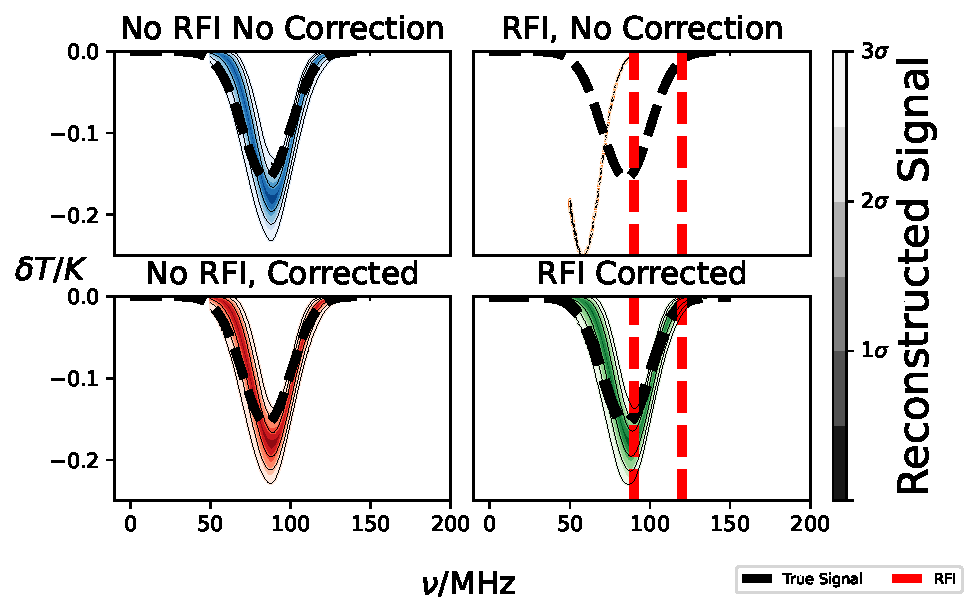
\includegraphics[width=\textwidth]{f_4pane_reach_sidebar.pdf}
    \caption{Showing the results when the RFI correction is applied on simulated data in the REACH data analysis pipeline.}\label{fig:reach_dual_plot}
\end{figure*}
Finally, we examine a real use case for this method. The REACH~\cite{de2022reach} radio telescope is designed to detect the faint 21cm signal from the Cosmic Dawn. This signal is estimated to be 5 orders of magnitude dimmer than the foreground, therefore a highly precise measurement is required. The REACH data analysis pipeline takes a Bayesian approach to antenna calibration, foreground modelling and chromaticity correction~\cite{anstey2021general}. As such it is a useful environment to test our RFI mitigation framework. The 21cm signal is expected to take the shape of an inverted Gaussian, so the model takes the form

\begin{equation}
    f(x) = A \exp{\bigg( -\frac{(x-\mu)^{2}}{2 \sigma^{2}}\bigg)}
\end{equation}
with center frequency $\mu$, standard deviation $\sigma$ and magnitude $A$ all free parameters. The four cases discussed in \cref{sec:toyex} are then examined, but this time on a simulated sky data set containing a 21cm signal with two RFI spikes injected. The evidences and subsequent log Bayes Factors are shown in~\cref{tab:tab2} below.
\begin{table}
\begin{center}
\begin{tabularx}{0.4\textwidth} { 
  | >{\raggedright\arraybackslash}X 
  | >{\centering\arraybackslash}X 
  | >{\raggedleft\arraybackslash}X | }
 \hline
    & No RFI & RFI \\
 \hline
 No Correction ($\log \mathcal{Z}$) & 296.0 $\pm$ 0.4  & -99525038.0 $\pm$ 0.5\\
 \hline
 Correction ($\log \mathcal{Z}$) & 295.4 $\pm$ 0.4 & 251.0 $\pm$ 0.4  \\
 \hline
 log Bayes Factor & =1.4 $\pm$ 0.6 & 99525289.0 $\pm$ 0.6 \\
 \hline
\end{tabularx}
\end{center}
\caption{Evidences when running the four cases described in~\cref{sec:reachex} and the subsequent Bayes factor.}
\label{tab:tab2}
\end{table}

The No RFI Correction and ground truth cases are very similar with the simpler (ground truth) case marginally preferred as expected. The RFI Corrected case is again similar with a slightly lower evidence due to the penalties incurred during the corrections. The above is also evident when viewing \cref{fig:reach_dual_plot}. The reconstructed signal is within $2\sigma$ of the true signal for all but the RFI No Correction case. 

\section{Conclusions}\label{sec:conclusions}
In this paper, which serves as a proof-of-concept, we show that RFI can be both flagged and corrected in a fully Bayesian sense at the likelihood level. This approach to RFI mitigation may be a highly effective tool for future radio telescopes, given the growing prevalence of modern data analysis pipelines taking a Bayesian approach and the need for a system that can be incorporated into these increasingly complex data analysis systems. Our methods can effectively perform inference on data hampered by RFI, as shown when tested on a simple toy model and also in a real use case in the pipeline of a global 21cm experiment, all as part of a single step Bayesian fitting process. 

In future works, it will be necessary to further examine to approximation made in \cref{eq:approx} to confirm that it is valid in other more complex scenarios. Further analysis is also required to assess the efficacy of this technique when compared to other modern RFI mitigation approaches. As mentioned in \cref{sec:rficorrtheory} we assume that each data point is separable and uncorrelated. It is unlikely that this is true for real data~\cite{wilensky2021improving}. Therefore, the case where data points are dependent on each other should be investigated in future works. Development is required to incorporate this method when applied to time integrated data and furthermore on different species of RFI, such as transient and broadband.

Our methodologies yield a means by which one can leverage their belief that certain parameters fit the data, therefore they will be useful in other fields. For example in the field of transient (Pulsar, Fast Radio Burst, etc) detection, RFI looks very similar in real space to the object of interest but very different in parameter space. One could thus leverage their belief in a Pulsars periodicity (for example) against similarly shaped (in real space) but non periodic RFI, generating a means by which the two phenomena can be distinguished from each other.

\section{Data Availability}
The methods described in this paper can be implemented into a Bayesian data analysis pipeline with just a few lines of code. An example can be found at \href{https://github.com/samleeney/Publications}{github.com/samleeney/publications}. All other data and codes related to these works are available on request.
\bibliographystyle{mnras}
\bibliography{ref.bib} % if your bibtex file is called example.bib

% Don't change these lines
\bsp	% typesetting comment
\label{lastpage}
\end{document}

% End of mnras_template.tex
